\section{Introduction}\label{sec-intro}

Software defined networking (SDN) 
%advocates for the separation of control and
%data planes in network devices, and provides a logically centralized platform
%to program data plane state~\cite{openflow,rethinking}.  This 
has opened the
door to rich network control applications that can adapt to changes in
network topology or traffic patterns more flexibly and more quickly than 
legacy control
planes~\cite{swan,b4,ananta,elastictree,softcell,zupdate,microte}.
%However, many important management applications in these domains, such
%as fast fail-over, reactive routing of latency-sensitive flows, and
%fine-grained DC traffic engineering~\cite{microte}, are stretching SDN's
%capabilities. These applications require the ability to reprogram data plane
%state at very fine time-scales to optimally meet their objectives.
However, to optimally satisfy network objectives, many important control 
applications require the ability to reprogram data plane state at very fine 
time-scales. For instance, fine-grained data center
traffic engineering requires routes to be set up within a few hundred
milliseconds to leverage short-term traffic
predictability~\cite{microte}. Similarly, setting up routes in
cellular networks (when a device becomes active, or during a handoff)
must complete within $\sim$30-40ms to ensure users can interact with
Web services in a timely fashion~\cite{softcell}.
%  It is important that SDN support such
% applications, otherwise operators will be forced to adopt expensive custom
% solutions alongside SDN (e.g., bandwidth reservation, custom
% hardware/protocols, etc.), which can undermine SDN's ``CapEx'' and ``OpEx''
% benefits.  \aaron{Should the preceding sentence be cut, because the proxy
% seems like ``custom hardware''?}

%For such applications, timely interaction between the logically
%central SDN control plane and network switches is crucial. 
Timeliness
is determined by: (1) the speed of control programs, (2) the latency
to/from the logically central controller, and (3) the responsiveness
of network switches in interacting with the controller---specifically,
in generating the necessary input messages for control programs, and
in modifying forwarding state as dictated by the programs. Robust control
software design and advances in distributed controllers~\cite{onix}
have helped overcome the first two issues. However, with the focus in
current/upcoming generations of SDN switches being on the flexibility
benefits of SDN w.r.t. legacy technology, the third issue has
not gained much attention. Thus, it is unknown whether SDN can
provide sufficiently responsive control to support the aforementioned
applications.


% Alarmingly, preliminary studies~\cite{ucsdpaper,oflops} and anecdotal
% evidence suggest that the latencies of switch control actions (\#3
% above) are significant. However, it is unclear what factors impact
% these latencies, what the underlying causes are, and whether the
% causes are fundamental to switch designs. 

To this end, we present a thorough systematic exploration of latencies in 
%\#3 above in
\numCombos types of production SDN switches from
\numVendors different vendors---Broadcom, Intel, and IBM---using a variety
of workloads. We investigate the relationship between switch design
and observed latencies using greybox probes and feedback from
vendors. Key highlights from our measurements are as follows: (1) We
find that {\em inbound latency}, i.e., the latency involved in the
switch generating events (e.g., when a flow is seen for the first
time) can be high---8 ms per packet on average on Intel. The
delay is particularly high whenever the switch is simultaneously
processing forwarding rules received from the controller. (2) We find
that {\em outbound latency}, i.e., the latency involved in the switch
installing/modifying/deleting forwarding rules provided by control
applications, is also high---3ms and 30ms per rule for insertion and
modification, respectively, in Broadcom. The latency crucially
depends on the priority patterns of both the rules being inserted and
those already in a switch's table. (3) We find significant differences in
latency trends across switches with different chipsets and firmware, pointing
to different internal optimizations.


%Wouldn't improvements in switch designs eliminate these latencies over
%time? 
These observations highlight two important gaps in current switch designs.
First, some of our findings show that poor switch software design
contributes significantly to observed latencies
(affirming~\cite{ucsdpaper,oflops}). We believe near term work
will address these issues; our measurements with an early release of
Broadcom's OpenFlow 1.3 firmware exemplify this. More crucially, our
measurements reveal latencies that appear to
be fundamentally rooted in hardware design: e.g., rules must be
organized in switch hardware tables in priority order, and
simultaneous switch control actions must contend for limited bus
bandwidth between a switch's CPU and ASIC. Unless the hardware
significantly changes---and our first-of-a-kind 
in-depth measurement study may engender such changes---we believe these latencies will
manifest even in next generation switches.

%Our measurements point out to switch manufacturers and chip developers the
%steps they need to take to eliminate these latencies. 

%We find that poor switch software design contributes significantly to the
%observed high latencies. However, pathological interactions between some rule
%priority input sequences and switch hardware table  heuristics for rule
%layout play a significant  role in inflating latency as well.  Crucially, the
%latter issue is  fundamental and may be hard to overcome.

%Informed by our measurements, we design a framework called Mazu that {\em
%leverages} the centralized view and global control in SDN to overcome or
%mitigate the impact of latencies, including both latencies from
%implementation-related causes and those from fundamental ones.

\iffalse
Since hardware upgrade cycles are 5+ years long (according to anecdotal
evidence), operators need immediately deployable solutions to 
mitigate these latencies while they wait for switch software and hardware to
appropriately evolve. 
\fi
%\fixme{I deleted the proxy}
%To this end, we design a framework called {\em Mazu}
%that leverages SDN's central view and global control.  To mitigate inbound
%latency arising from bus bottlenecks in switches,
%arising from data plane packet arrivals, 
%Mazu redirects relevant packets to a fast proxy that generates the 
%necessary messages for the controller.
%  By
% using a commodity machine, with high NIC-to-CPU bandwidth and a fast
% CPU, we are able to
%This virtually eliminates inbound latency and saves
%switch resources for rule updates.
%By leveraging a fast commodity processor and decoupling inbound and outbound
%actions, this eliminates inbound latency.
%\fixme{i changed here}

\iffalse
Many SDN applications already avoid (or minimize their dependence on) packet-in 
messages, thereby mitigating the impact of inbound latency. In contrast, rule
installations/updates are an intrinsic part of SDN applications, which makes
outbound latency more challenging, and important, to address.
\fi
%\aaron{This sentence needs to be re-worded: In this paper, we propose three techniques to mitigate the latency of existing hardware's outbound operation, 
%which is intrinsically linked to switch
%design (especially hardware) and more widely used in production:}
\iffalse
In this paper, we propose three techniques to mitigate the outbound latencies
imposed by current switches:
{\em Flow engineering} (FE) leverages our empirical latency models to compute
paths such that the latency of installing forwarding state at any
switch is minimized. 
%\aaron{Dionysus does similar things as FE for consistent
%    updates. Do we provide more than Dionysus?} 
{\em Rule
  offloading} (RO) computes strategies for opportunistically
offloading installation of some forwarding state to downstream switches.
Finally, {\em rule reordering} (RR) sends rule installation
requests in an order that is optimal for the switch in question. By reducing
installation latency per switch (FE + RR) and enabling network-wide parallel
updates (RO), 
%\aaron{Doesn't FE also enable parallel updates?}
rule updates can finish much faster.
%, and the impact of outbound latency is minimized.

 We evaluate these techniques for fast fail-over and responsive
 traffic engineering applications under various settings. Depending on
 the topology and the nature of rules in switches, we find that
outbound latencies can render SDN incapable of supporting such
applications. In contrast, 
our techniques can
 improve the time taken to update network state in these scenarios by factors
 of 1.6-5X, which we argue makes SDN-based control suitably responsive for these
 settings.
\fi
% \aditya{what about priority insertion}

% \aditya{this will go: Our final technique, multipath probing,
%  sets up multiple paths in parallel so that data plane packets can be
%  switched in hardware as soon as one path completes its setup.  This
%  mechanism deals with unexpected delays imposed by switch CPU (e.g.,
%  due to CPU  processing
%  of other tasks such as polling statistics) and hardware (e.g., due to
%  TCAM reorganization).}

%  \aditya{some sentences
%   in this para will have to
%   be  rewritten}

% \aditya{rest is to do}

% % Finally, we control the actual
% % installation of flows at edge and core switches by reordering them
% % according to priority.\aditya{check this XXX}\marina{is there a
% %   batching of the rules as well before determining order}

% \iffalse

% In some situations, the t\_out latencies may be impacted by other
% factors that cannot be controlled; e.g., when an application is
% attempting to reactively install routes while another is reading
% statistics from existing switches. While the above approaches help
% reduce latency somewhat in such situations, there is still enough
% variation in the latencies that flows can face.
%  meeasurements do not unearth. To account for these, we introduce an
%  opportunistic multipath probing scheme that explores up to
%  $k$ candidate paths between a source destination pair \marina{these paths are based on existing rule sets in the switches?}, taking
%  into account potential interference across pairs. The schemes selects
%  one path per pair such that the t\_out delay experienced by all pairs
%  is minimized. \aditya{need to finish. need a lot more detail.}


 
% However, it is not clear what factors cause such high latencies and
% whether the causes are fundamental to design. Equally importantly, 

% arise
% However, it is not
% known why the latencies arise, whether the underlying causes are
% fundamental However, it is not known how the latencies manifest under
% various workload conditions and across a variety of platforms, what
% underlying issues contribute to them, and whether these issues are
% fundamental to switch designs today.


% % While SDN has certainly made the control planes richer and more
% % robust, it introduces a new complexity: the control plane can impact
% % the performance of the data plane on fine time-scales. 

% %  twist to how the control plane affects
% % data plane performance. In traditional networks, the control plane's
% % poor adaptation lead to the data plane doing useless work (e.g.,
% % packets looping during convergence) or being not fully utilized. In
% % SDNs, however, the data plane performance is impacted on fine
% % time-scales because of 

% % challenges

% But exactly how responsive is SDN-based network control? Consider the
% example where an OpenFlow-based SDN application is trying to
% reactively establish routes for flows within the data center, e.g., in
% response to a failure. The actions involved are shown in Figure XXX
% for a simplified network with a single switch.\marina{Is this Fig same
%   as Fig 1, also include numbering on fig to show sequence of flow set
%   up process} Notice that the actual forwarding for the flow in
% question does not begin until t\_in + t\_out seconds. If the latency
% introduced by the network is ignored, then t\_in and t\_out are driven
% purely by the ability of SDN switches to quickly execute SDN-related
% actions.

% Most existing SDN approaches assume that these latencies are
% negligible. This would be possible in a world where SDN switch
% software and chip designs are highly optimized to support SDN-based
% actions. In practice, however, poor software designs, unoptimized
% hardware paths, and fundamental traits of memory hardware conspire to
% cause the latencies to be significantly higher!

% In~\figref{openflow_switch_delay}, we show a deeper view into an SDN
% switch, various actions the switch takes, and how they contribute to
% t\_in and t\_out. As the figure indicates, the latencies t\_in and
% t\_out depend on key aspects of the switch's design including how the
% switch software processes different messages, the software's
% interaction with the switch hardware table (typically a TCAM), and the
% corresponding actions taken by the hardware table's SDK. These aspects
% may be exercised to different extents based on switch workload, such
% as the nature of the rule being installed (simple 5-tuple based vs
% complex rule based on the entire OpenFlow 10-tuple), the rule's
% priority relative to those already installed, size of the currently
% installed rule base, rate at which the controller is simultaneously
% pushing other rules to the switch and the nature of those rules, etc.

% To date, not much attention has been paid to estimating these
% latencies in the wild under various workloads, and analyzing the
% impact of switch designs on the latencies. \marina{Place UCSD paper into context} Understanding these is
% crucial to how SDN is used: it can inform operators on whether certain
% SDN approaches (such as the reactive failure avoidance approach above)
% can offer close to the promised benefits given current switches on the
% market. It can also inform them on how best to avoid or mitigate the
% impact of the latencies on their applications. To switch and chip
% vendors, it can highlight what aspects of their software and SDK
% designs can be improved to support faster actions.
% % how to alter SDN switch designs where possible to address the latencies, and how to develop SDN applications that modulate switch workloads to avoid being impacted by the latencies.

% \begin{figure}[!tb]
% \centering
% %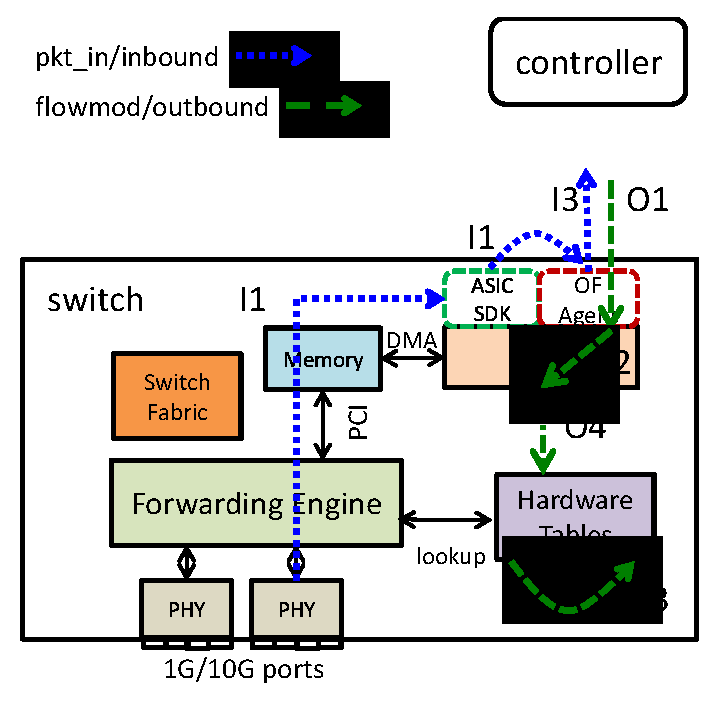
\epsfig{file=./figs/openflow_switch_illustrate.eps,width=0.4\textwidth}
% 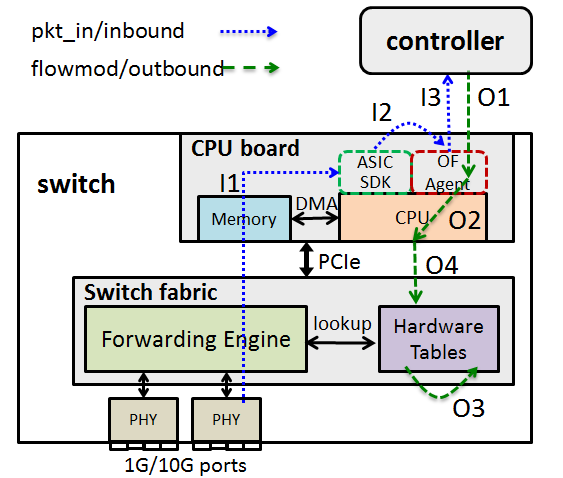
\includegraphics[width=3.5in]{figs/openflow_switch.PNG}
% \caption{Illustration of the t\_in and t\_out delay in an openflow switch.}\label{openflow_switch_delay}
% \end{figure}

% The first contribution of this paper is a systematic exploration of
% latencies in production SDN switches. We study switches from XXX
% \aditya{fill} different vendors under a variety of scenarios that
% carefully isolate the impact of different workload parameters on
% observed latencies. Further, we investigate the relationship between
% switch designs and observed latencies using both active greybox probes
% and feedback from hardware vendors. Key highlights from our
% measurements are as follows: (1) We find that t\_in delays can be as
% high as XXXXms.\aditya{fill} In some cases, poor software support for
% handling \packetin\ message may be an underlying cause, but we note
% that t\_in is always high whenever switch software is also processing
% \packetout\ and \flowmod\ messages. (2) We find that t\_out is
% unusually high as well: for example, inserting a burst of 50 rules
% into a switch based on the Broadcom chipset can take up to 100ms. TCAM
% hardware can support very fast updates, so this delay appears to arise
% primarily from switch software issues. \marina{such as when and what types of rules get puhsed into the TCAM} (3) Priorities can have a
% significant impact: inserting high priority rules into a table
% containing lower priority rules can take as long as XXXs.\aditya{fill}
% This is due to the memory chip's SDK rearranging rules in order of
% priority.

% Crucially, most of the root causes of the latencies are often not
% fundamental and arise due to poor switch software design. Only one
% root cause -- rule rearrangment in face of priorities -- appears to be
% linked to the hardware. A natural question to ask is whether switch
% vendors will improve their software such that most of the latencies we
% observe would go away. We don't believe this is likely: switch vendors
% will not put in the software design effort unless they see the outcome
% as a differentiator. Customers today continue to make purchase
% decisions mostly based on line speeds and perhaps flow table sizes,
% and hence it is likely that we're stuck at least in the near future
% with switch designs that are similar to what we have today.

% \fi
